
\begin{frame}[fragile]{Algèbre relationnelle\,: expressions algébriques}

Par \alert{composition} on exprime avec l'algèbre toutes les requêtes relationnelles
que l'on peut aussi exprimer (plus naturellement) avec la logique.

\vfill

Dans cette session, des exemples d'\alert{expressions algébriques} courantes

\begin{redbullet}
  \item Composition de sélections
  \item Jointures
  \item Différence
  \item Et même la quantification universelle
\end{redbullet}

\vfill

\begin{blocgauche}
\alert{Ces diapositives correspondent au support en ligne disponible sur
le site \url{http://sql.bdpedia.fr/}}
\end{blocgauche}

\end{frame}


\begin{frame}{Composition de sélection }

La \alert{conjonction} de critères s'obtient en composant des sélections

     $$\sigma_{capacit\acute{e}>100}(\sigma_{type='H\hat{o}tel'}(Logement))$$
     
\vfill

On acceptera de l'écrire

   $$\sigma_{capacit\acute{e}>100 \land type='H\hat{o}tel'}(Logement)$$

\vfill

\alert{L'union} est l'équivalent en algèbre de la \alert{disjonction} logique.

$$ \sigma_{capacit\acute{e}>100}(Logement) \cup \sigma_{lieu='Corse'}(Logement)$$


\vfill

Peut s'écrire

    $$\sigma_{capacit\acute{e}>100\ \lor\  lieu='Corse'}(Logement)$$
\end{frame}

\begin{frame}{Composition de sélection, suite }

La différence permet d'exprimer l'opérateur $\not=$.

     $$\sigma_{capacit\acute{e}>100}(Logement) - \sigma_{lieu='Corse'}(Logement) $$
     
\vfill

On acceptera de l'écrire

   $$\sigma_{capacit\acute{e}>100 \land \neg (lieu ='Corse')}(Logement) $$

\vfill

En résumé, on peut écrire la sélection en exprimant les critères avec une formule
$F$ du calcul propositionnel,  $\sigma_F(R)$


\vfill

\alert{Attention} à la négation: voir plus loin.
\end{frame}


%%%
\begin{frame}{Requêtes conjonctives}

Toute requête s'écrivant avec $\sigma$, $\pi$, $\times$ (et donc $\Join$).

\vfill
Nom des logements en Corse :  
  
    $$\pi_{nom}(\sigma_{lieu='Corse'}(Logement))$$
    
\vfill

Code des logements où l'on pratique la voile.
       
    $$\pi_{codeLogement}(\sigma_{codeActivit\acute{e}='Voile'}(\text{Activité}))$$

\vfill

Nom et prénom des clients corses
          
    $$\pi_{\text{nom,prénom}}(\sigma_{\text{région}='Corse'}(Voyageur))$$
\end{frame}



%%%
\begin{frame}{Jointures}
Nom des clients qui sont allés à Tabriz
  
    $$ \pi_{nom} (\text{Voyageur} \Join_{idVoyageur=idVoyageur} (\sigma_{codeLogement='ta'} (\text{Séjour})))$$

\vfill
Quels lieux a visité le client 30
    
    $$\pi_{lieu} (\sigma_{idVoyageur=30} (\text{Séjour}) \Join_{codeLogement=code} \text{Logement})$$
 
\vfill

Nom des clients qui ont eu l'occasion de faire de la voile. En deux étapes.

\vfill
$R1 :=  \texttt{Séjour} \Join_{codeLogement=codeLogement} (\sigma_{codeActivit\acute{e}='Voile'}(\texttt{Activité}))$
\vfill
$\pi_{nom} (\texttt{Voyageur} \Join_{idVoyageur=idVoyageur} R1)$
   
\end{frame}



%%%
\begin{frame}{La négation}


S'exprime en algèbre avec la \alert{différence}. 

\vfill
Codes des logements qui \alert{ne proposent pas}
de voile

$$\pi_{code}(\text{Logement}) - \pi_{codeLogement}(\sigma_{codeActivit\acute{e}='Voile'}(\text{Activité}))$$

\vfill

\alert{Raisonnement}: je prends \alert{tous} les logements \alert{moins} ceux qui proposent de la voile.

\vfill
\begin{blocgauche}
\alert{Très peu pratique} si on compare au \sqlkw{not exists}: 
la différence ne s'applique que sur des relations ayant \alert{le même schéma}.
\end{blocgauche}

\end{frame}



\begin{frame}{Logique ou fonctionnel, quel langage?}

\vspace*{0.3cm}

On soumet une requête SQL, et après? 

\vfill


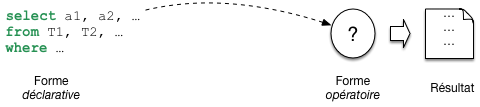
\includegraphics[width=10cm]{../../figures/exec-optim-1}

\vfill
\begin{blocgauche}
On exprime la requête de manière \alert{déclarative}, le système
doit trouver une méthode d'évaluation.
\end{blocgauche}
\end{frame}


\begin{frame}{Expression logique, évaluation fonctionnelle}

\vspace*{0.3cm}
Le système peut produire une expression algébrique pour toute requête SQL.

\vfill


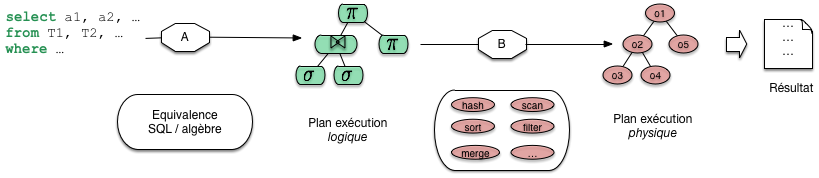
\includegraphics[width=10cm]{../../figures/exec-optim-3}

\vfill
\begin{blocgauche}
Il reste à trouver les bons algorithmes, à utiliser correctement les ressources
de calcul: c'est pour les administrateurs.
\end{blocgauche}
\end{frame}
\begin{frame}{À retenir}

L'algèbre est un langage relationnel \alert{équivalent} à la logique formelle.
\vfill

\begin{redbullet}
  \item  On peut exprimer \alert{toutes} les requêtes en algèbre.

  \item Il existe une syntaxe SQL pour \alert{toutes} les requêtes algébriques
  
  \item Le style est celui de la programmation; moins clair, moins accessible à un non-programmeur,
     moins proche de l'expression ``naturelle'' de la requête.
     
   \item Peut s'effectuer en plusieurs étapes pour une meilleure clarté.
\end{redbullet}

\vfill
\begin{blocgauche}
L'algèbre était conçue à l'origine pour définir \alert{l'exécution} 
des requêtes, pas leur \alert{expression}.
\end{blocgauche}
\end{frame}
